\documentclass{article}%
\usepackage[T1]{fontenc}%
\usepackage[utf8]{inputenc}%
\usepackage{lmodern}%
\usepackage{textcomp}%
\usepackage{lastpage}%
\usepackage{geometry}%
\geometry{left=3cm,right=3cm,bottom=2cm,top=1cm}%
\usepackage[russian]{babel}%
\usepackage{amsmath}%
\usepackage{amssymb}%
\usepackage{amsfonts}%
\usepackage{mathtext}%
\usepackage{graphicx}%
%
%
%
\begin{document}%
\normalsize%
\begin{center}%
\vspace*{\fill}%
{\LARGE\textbf{Лабораторная работа № 3.10: \\ Изучение свободных затухающих электромагнитных колебаний}}\\[1cm]%
{\Large Исхаков Камиль Фархатович}\\[1cm]%
{\Large \today}%
\vspace*{\fill}%
\end{center}%
\newpage%
\section{Основные формулы}%
\label{sec:}%
\begin{itemize}    \item $\lambda$ --- логарифмический декремент затухания;    \item $U_i$ --- амплитуда напряжения на конденсаторе в момент времени $i$;    \item $U_{i+n}$ --- амплитуда напряжения на конденсаторе в момент времени $i+n$;    \item $n$ --- число полных периодов, между моментами времени $i$ и $i+n$;    \item $\beta$ --- коэффициент затухания;    \item $T$ --- период колебаний;    \item $R$ --- полное сопротивление контура;    \item $L$ --- индуктивность катушки;    \item $C$ --- емкость конденсатора;    \item $Q$ --- добротность контура;    \item $R_M$ --- добавочное сопротивление магазина;    \item $R_0$ --- собственное сопротивление контура;    \item $R_{\text{крит}}$ --- критическое сопротивление контура.\end{itemize}\begin{equation*}    \lambda = \frac{1}{n}\ln{\frac{U_i}{U_{i+n}}}\end{equation*} \begin{equation*}    \lambda = \beta T = \frac{R}{L}\frac{\pi}{\sqrt{\frac{1}{LC} - \frac{R^2}{4L^2}}}\end{equation*} \begin{equation*}    R = R_M + R_0\end{equation*} \begin{equation*}    R_0 = -R_M|_{\lambda = 0}\end{equation*} \begin{equation*}    Q = \frac{2\pi}{1 - e^{-2\lambda}}\end{equation*} \begin{equation*}    R_{\text{крит}} = 2\sqrt{\frac{L}{C}}\end{equation*} \begin{equation*}    T = 2\pi\sqrt{LC}\end{equation*}%


\begin{figure}[h!]%
\centering%
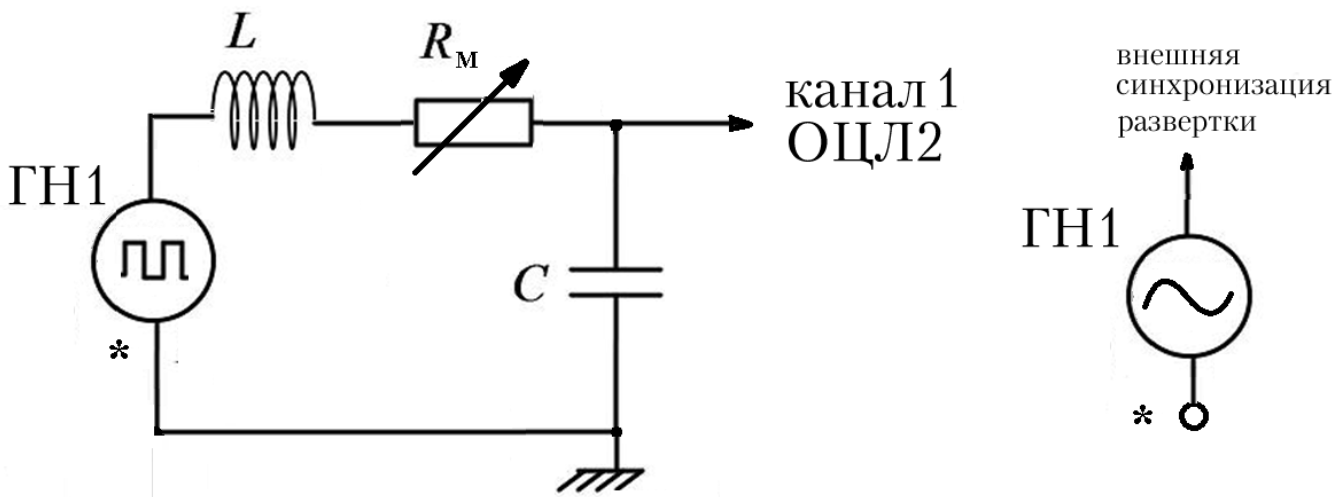
\includegraphics[width=300px]{lab_3_10_p1.png}%
\caption{Принципиальная электрическая схема установки}%
\end{figure}

%
\section{Результаты эксперимента}%
\label{sec:}%


\begin{table}[h!]%
\centering%
\begin{tabular}{|c|c|c|c|c|c|c|c|c|}%
\hline%
$R_M$, Ом&$T_M$, мс&$2 U_i$, дел&$2 U_{i+n}$, дел&$n$&$\lambda$&$Q$&$R$&$L$\\%
\hline%
0.00&86.00&6.08&2.28&3&0.33&13.09&77.54&12.21\\%
\hline%
20.00&86.00&5.36&1.52&3&0.42&11.05&97.54&11.71\\%
\hline%
40.00&86.00&4.92&1.08&3&0.51&9.88&117.54&11.74\\%
\hline%
60.00&86.00&4.40&0.72&3&0.60&8.97&137.54&11.28\\%
\hline%
80.00&86.00&3.84&0.52&3&0.67&8.53&157.54&12.13\\%
\hline%
100.00&86.00&3.52&0.36&3&0.76&8.04&177.54&11.85\\%
\hline%
300.00&86.00&1.32&0.12&2&1.20&6.91&377.54& – \\%
\hline%
\end{tabular}%
\caption{Измерения 1}%
\end{table}

%
Среднее значение индуктивности: 11.82 мГн\\%
Погрешность среднего значения индуктивности: $0.16$ мГн\\%
Для $R = $77.54 посчитаем добротность $Q = \frac{1}{R} \cdot \sqrt{\frac{L}{C}}$= 13.18 \\%
Критическое сопротивление $R = 1087$ Ом \\%
$R_0 = $ 77.54 Ом \\%
Теоретическое значение критического сопротивления $R$ при $L = 11$ мГн: 1414.21 Ом\\%
Эксперементальное значение сдвига фаз: $\delta_{\text{эксп}} = $ 1.64\\%
Теоретическое значение сдвига фаз: $\delta_{\text{теор}} = $ 1.60\\%


\begin{table}[h!]%
\centering%
\begin{tabular}{|c|c|c|c|c|c|}%
\hline%
$C$, мкФ&$T_{\text{эксп}}$, мс&$T_{\text{теор}}$, мс&$\delta T, \%$&$T_{\text{томп}}$, мс&$T_{\text{теор}}/T_{\text{эксп}}$\\%
\hline%
0.022&86.00&101.47&15.24&101.32&1.18\\%
\hline%
0.033&110.00&124.36&11.54&124.10&1.13\\%
\hline%
0.047&132.00&148.54&11.14&148.10&1.13\\%
\hline%
0.47&418.00&482.98&13.45&468.33&1.16\\%
\hline%
\end{tabular}%
\caption{Измерения 2}%
\end{table}

%


\begin{figure}[h!]%
\centering%
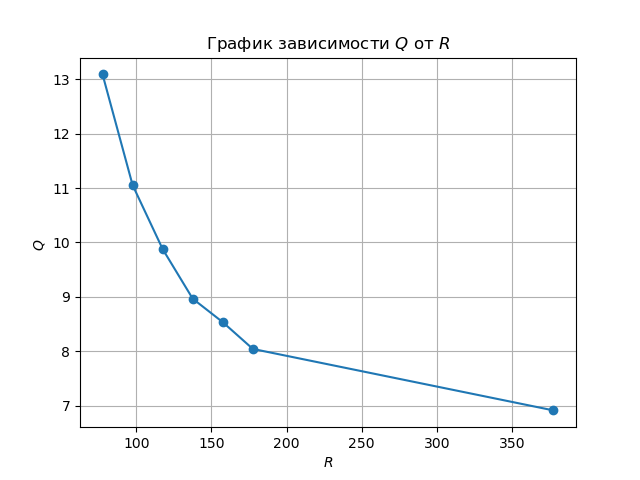
\includegraphics[width=300px]{Q_vs_R.png}%
\caption{График зависимости $Q$ от $R$}%
\end{figure}

%


\begin{figure}[h!]%
\centering%
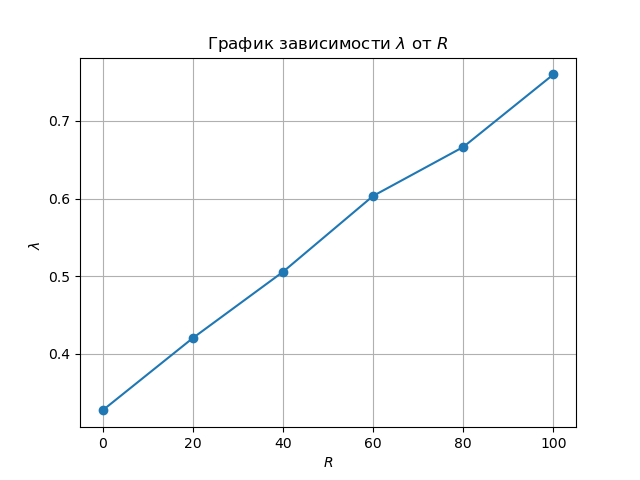
\includegraphics[width=300px]{Lambda_vs_R.png}%
\caption{График зависимости $\lambda$ от $R$}%
\end{figure}

%


\begin{figure}[h!]%
\centering%
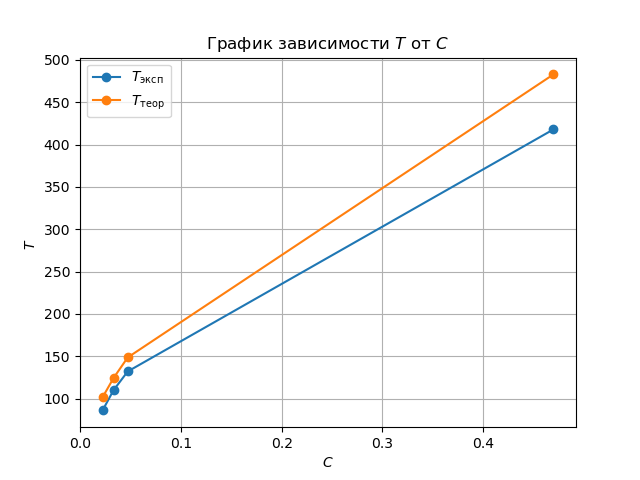
\includegraphics[width=300px]{T_vs_C.png}%
\caption{График зависимости $T$ от $C$}%
\end{figure}

%


\begin{figure}[h!]%
\centering%
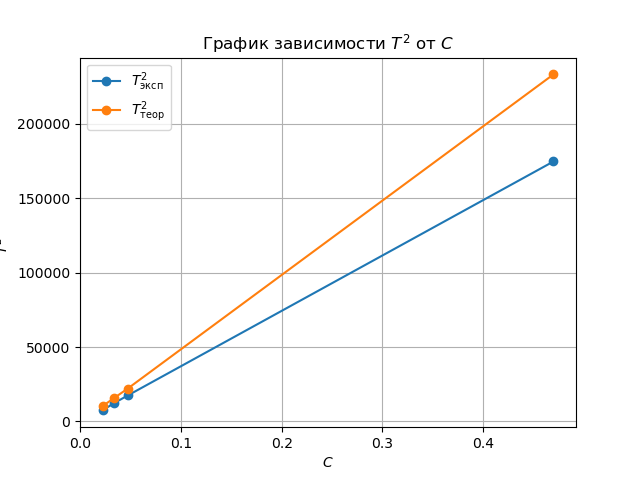
\includegraphics[width=300px]{T^2_vs_C.png}%
\caption{График зависимости $T^2$ от $C$}%
\end{figure}

%


\begin{figure}[h!]%
\centering%
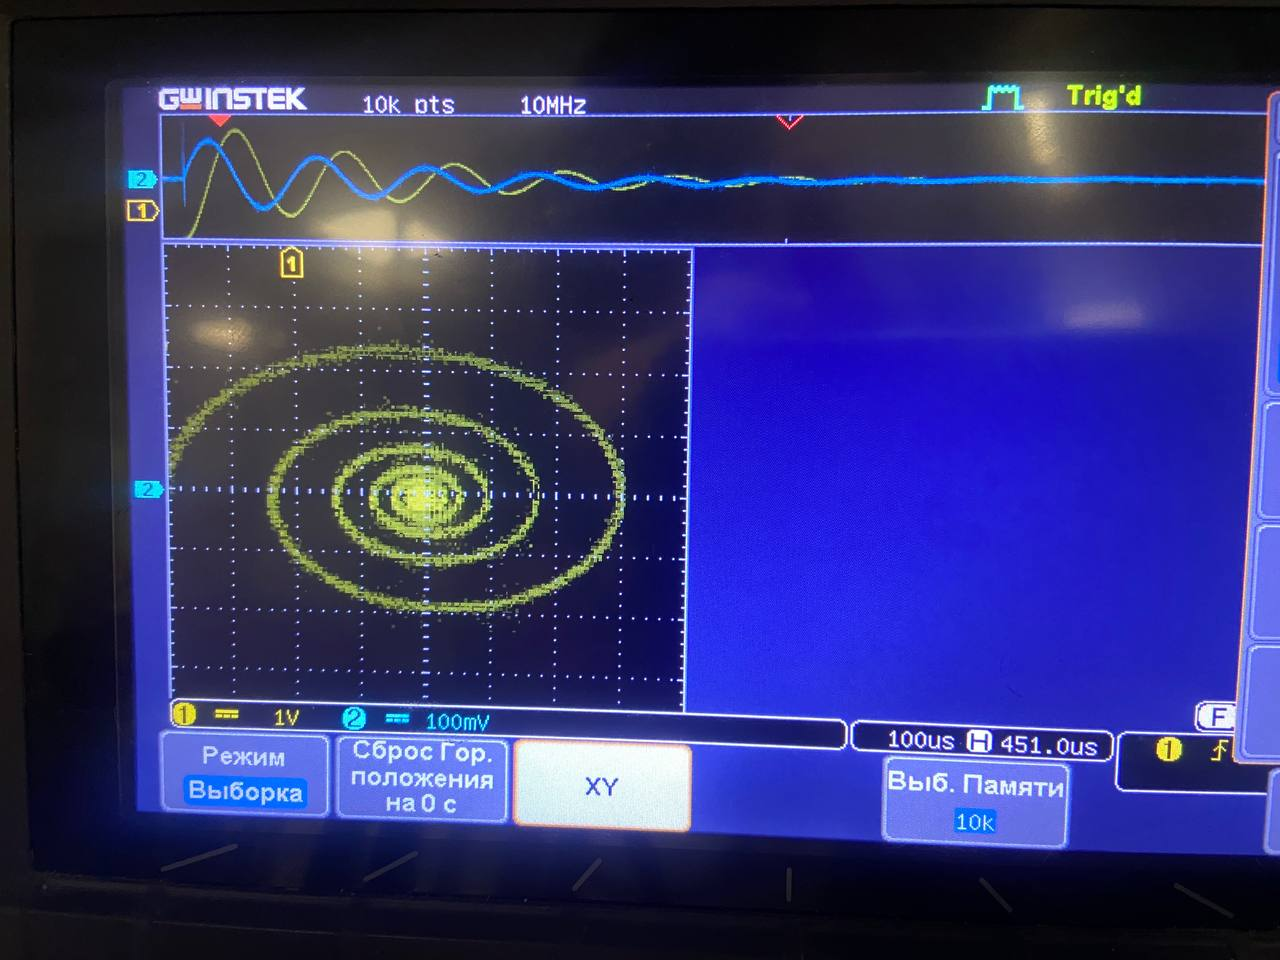
\includegraphics[width=300px]{lab_3_10_petly.jpg}%
\caption{Фазовая кривая $I(U)$}%
\end{figure}

%
\newpage%
\section{Выводы}%
\label{sec:}%
Расчеты показали, что полученные экспериментальные значения периода, логарифмического декремента затухания, добротности контура и фазового сдвига согласуются с теоретическими предсказаниями, хотя наблюдаются некоторые расхождения, которые могут быть обусловлены неидеальностями экспериментальной установки.

%
\end{document}